\documentclass[sigconf]{acmart}
% ---------------------------------------------------------------- cleaning (as in the course sample)
\settopmatter{printacmref=false, printfolios=false}
\renewcommand\footnotetextcopyrightpermission[1]{}
\pagestyle{plain}
\setcopyright{none}
\acmDOI{}
\acmConference{}{}{}
\acmBooktitle{}
\acmPrice{}
\acmISBN{}

\usepackage{booktabs}
\usepackage{graphicx}
\usepackage{amsmath}
\setlength{\emergencystretch}{2em}
\newcommand{\RQ}[1]{\textbf{RQ#1}}

\begin{document}
\title{MajorMatch: Evaluating Similarity- and Profile-Based Recommenders for University Majors}
\titlenote{Code, data and results: \url{https://github.com/yashwanth973/CSC503}}

\author{Thai Hung Vuong}
\affiliation{\institution{University of Victoria}\country{Canada}}
\email{thaihungvuong@uvic.ca}
\author{Brendan Wong}
\affiliation{\institution{University of Victoria}\country{Canada}}
\email{brendanwong@uvic.ca}
\author{Robert Legassicke}
\affiliation{\institution{University of Victoria}\country{Canada}}
\email{roblegs@uvic.ca}
\author{Yashwanthkrishna Nagharaj}
\affiliation{\institution{University of Victoria}\country{Canada}}
\email{yashwanthk@uvic.ca}

\begin{abstract}
We evaluate MajorMatch's $k$-NN (Jaccard) and Multinomial Naive Bayes (MNB) recommenders against five baselines on our survey and on a controlled benchmark of varying signal strength. On the survey every model is at chance, as its features are unrelated to the major. On the benchmark all models learn: Logistic Regression is best and MNB ranks almost as well. Code, data and results (MIT license): \url{https://github.com/yashwanth973/CSC503}.
\end{abstract}

\keywords{recommender systems, major selection, evaluation, k-NN, naive Bayes}
\maketitle

% =====================================================================
\section{Introduction}
MajorMatch maps a student's 12 binary skills and clubs to a ranked list of majors (Milestone~3). Our contribution is a \emph{new application} of similarity-based ($k$-NN, as in CoDeRS~\cite{rances2026coders}) and profile-based (MNB) recommenders to major selection, so we ask how effective they are there against conventional classifiers under one shared protocol.

% =====================================================================
\section{Research Questions}
\noindent\RQ{1}: \emph{Do our recommenders outperform conventional classifiers?} This tests whether our M3 design pays off; we compare against five baselines on both datasets' final test sets.

\noindent\RQ{2}: \emph{How sensitive are they to $k$ and $\alpha$?} This checks the M3 defaults ($k{=}7$, $\alpha{=}1$) via mean 5-fold CV macro-F1 over each grid.

\noindent\RQ{3}: \emph{Is performance consistent across datasets of different signal strength?} This separates method failures from data failures; we sweep the benchmark noise $\eta$ from 0 (clean) to 1 (survey-like).

\begin{figure*}[t]
\centering
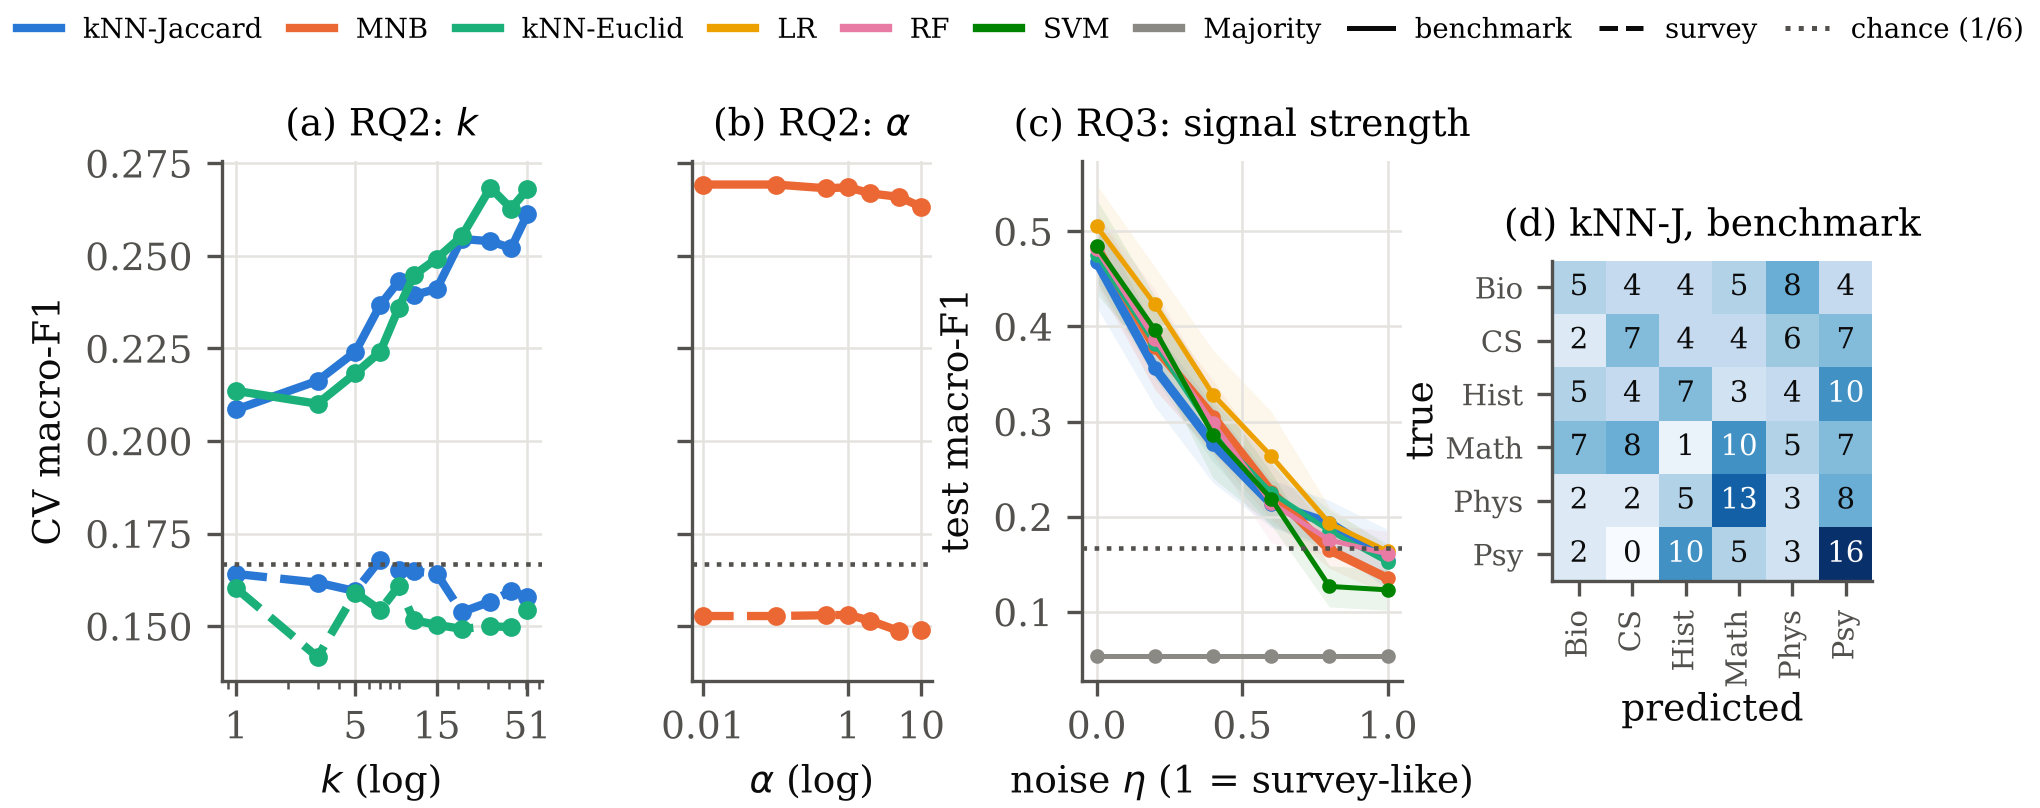
\includegraphics[width=\textwidth]{Images/evaluation_panels.png}
\caption{(a, b) \RQ2: mean 5-fold CV macro-F1 over $k$ and $\alpha$ (solid: benchmark, dashed: survey). (c) \RQ3: test macro-F1 (mean$\pm$std, 5 seeds) as benchmark noise $\eta$ grows. (d) Confusion matrix of kNN-Jaccard on the benchmark test set (seed 2026).}
\label{fig:panels}
\end{figure*}

% =====================================================================
\section{Datasets}
\textbf{Survey (real).} Our survey of 1000 students (12 binary features, 6 majors) is the only data on our target population, but a $\chi^2$ test finds no feature associated with the major ($p{>}0.19$ for all 12).

\textbf{Benchmark (controlled).} To test the methods when signal \emph{exists}, we draw 1000 students: a major with the survey's class shares, then feature $j$ with probability $(1{-}\eta)\,\mathrm{prof}_{m,j}+\eta\,\mathrm{prev}_j$, where $\mathrm{prof}$ is a documented high/medium/low profile per major (e.g., CS: Programming) and $\mathrm{prev}_j$ the survey prevalence, so $\eta{=}1$ reproduces the survey. The main benchmark uses $\eta{=}0.5$, \emph{fixed before any result was seen}; all models get identical data (Table~\ref{tab:data}).

\begin{table}[t]
\caption{Dataset statistics (benchmark at $\eta{=}0.5$, seed 2026).}\label{tab:data}
\footnotesize
\begin{tabular}{@{}lcc@{}}
\toprule
 & Survey (real) & Benchmark \\ \midrule
Students / features / majors & 1000 / 12 / 6 & 1000 / 12 / 6 \\
Missing values; source & 0; team survey & 0; generated \\
Class share (min--max) & 14.9--17.9\% & 14.9--19.3\% \\
Avg.\ features per student & 7.07 & 6.50 \\
Feature--major association & none ($p{>}0.19$) & by design \\ \bottomrule
\end{tabular}
\end{table}

% =====================================================================
\section{Baselines}
All baselines use scikit-learn~\cite{pedregosa2011sklearn} and rank majors by predicted probability. \textbf{kNN-Euclid}~\cite{cover1967knn}: votes of the $k$ nearest students by Euclidean distance, $k\in\{1,\dots,51\}$; isolates our Jaccard choice.
\textbf{LR}~\cite{cox1958lr}: multinomial, $C\in\{0.01,\dots,100\}$; a parametric linear rival.
\textbf{RF}~\cite{breiman2001rf}: depth $\in\{3,5,10,\infty\}$, $\{100,300\}$ trees; models feature interactions.
\textbf{SVM}~\cite{cortes1995svm}: RBF kernel, $C\in\{0.1,1,10\}$, with Platt-scaled probabilities~\cite{platt1999}.
\textbf{Majority}: ranks majors by frequency; the floor. Ours search $k\in\{1,\dots,51\}$, $\alpha\in\{0.01,\dots,10\}$.

% =====================================================================
\section{Evaluation Strategy and Metrics}
Each dataset is split into a stratified 80\% development / 20\% final test set. Stratified 5-fold CV on the development set, with \emph{the same folds for every model}, scores each configuration; the best mean CV macro-F1 is refit on the whole development set and tested \emph{once}. This is repeated for seeds 2026--2030 (mean$\pm$std).
\emph{Metrics:} macro-F1 of the top-1 major is primary (balanced classes, each counts equally); top-2 accuracy matches what a student sees; macro one-vs-rest AUC measures ranking; plus a confusion matrix and fit+predict time.

\begin{table}[t]
\caption{\RQ1: final-test results, mean over 5 seeds (macro-F1 $\pm$ std). Bold: best per column; chance: F1 0.167, top-2 0.333, AUC 0.5.}\label{tab:rq1}
\footnotesize
\resizebox{\columnwidth}{!}{%
\begin{tabular}{@{}l|ccc|ccc|r@{}}
\toprule
 & \multicolumn{3}{c|}{Survey (real)} & \multicolumn{3}{c|}{Benchmark ($\eta{=}0.5$)} & \\
Model & F1 & top-2 & AUC & F1 & top-2 & AUC & ms \\ \midrule
kNN-Jaccard (ours) & .171$\pm$.020 & .303 & .506 & .244$\pm$.034 & .471 & .612 & 31 \\
MNB (ours) & .138$\pm$.017 & .329 & .500 & .265$\pm$.036 & .522 & .670 & 7 \\ \midrule
kNN-Euclid & .164$\pm$.017 & .358 & .508 & .275$\pm$.039 & .493 & .636 & 15 \\
LR & \textbf{.173}$\pm$.028 & .337 & .493 & \textbf{.297}$\pm$.035 & \textbf{.541} & \textbf{.674} & 15 \\
RF & .155$\pm$.023 & .349 & .506 & .271$\pm$.033 & .496 & .654 & 362 \\
SVM & .159$\pm$.030 & \textbf{.375} & \textbf{.516} & .262$\pm$.033 & .520 & .648 & 132 \\
Majority & .051$\pm$.000 & .355 & .500 & .053$\pm$.001 & .368 & .500 & 7 \\ \bottomrule
\end{tabular}}
\end{table}



% =====================================================================
\section{Results and Discussion}
\textbf{\RQ1.} On the \emph{survey} (Table~\ref{tab:rq1}) no model differs from chance (F1 0.14--0.17, AUC 0.49--0.52), and none beats always recommending the two most frequent majors (top-2 0.355). \emph{Why:} its features carry no information about the major, so the model ordering there is noise. On the \emph{benchmark} every model learns (F1 0.24--0.30, AUC 0.61--0.67), but ours do \emph{not} beat the baselines: LR is best and beats MNB on all 5 seeds (+0.032 F1). MNB nevertheless ranks almost as well as LR (AUC 0.670 vs.\ 0.674, top-2 0.522 vs.\ 0.541) at half LR's cost (7 vs.\ 15\,ms), making it the fastest learned model; RF is the slowest (362\,ms) without gaining accuracy. \emph{Why:} benchmark features are independent given the major, so the true log-odds are linear in $\mathbf{x}$ (LR's family), while MNB uses only features a student \emph{has} and ignores informative absences. kNN-Jaccard is the weakest learner (0.244). Euclidean distance beats it on 4 of 5 seeds, contradicting our M3 assumption that shared absences are uninformative (two students both \emph{lacking} Debate Club are less likely in History). Its errors (Fig.~\ref{fig:panels}d) concentrate where profiles overlap: Physics$\to$Math (13), History$\leftrightarrow$Psychology (10 each).

\textbf{\RQ2.} On the benchmark (Fig.~\ref{fig:panels}a) $k$-NN improves with $k$, from 0.21 at $k{=}1$ to 0.26--0.27 for $k{\ge}21$, as more neighbours average out feature noise; our M3 default $k{=}7$ (0.237) is too small, and CV picked $k\in[11,51]$. On the survey no $k$ helps. MNB (Fig.~\ref{fig:panels}b) is insensitive to $\alpha$ (CV F1 varies by 0.006 over three orders of magnitude): with $\sim$130 students per major, counts $c_{m,j}$ are in the hundreds, so $\alpha{\le}10$ barely changes $\theta$; $\alpha{=}1$ is safe.

\textbf{\RQ3.} Performance is \emph{consistent in ordering, not in level} (Fig.~\ref{fig:panels}c). All models decline monotonically with $\eta$ and collapse to chance (0.12--0.16) at $\eta{=}1$, reproducing the survey's numbers with different students: the survey failure lies in the data, not our implementation. LR leads at every level (beating MNB in 25 of 30 runs), MNB stays within 0.02--0.04 of it, and kNN-Jaccard trails on clean data (0.468 vs.\ 0.505). Even at $\eta{=}0$ F1 is only $\approx$0.5, as STEM profiles overlap by design.

\textbf{Threats to validity.} The benchmark profiles are our assumptions and its independence favours linear models; real data with interactions could favour $k$-NN or RF. With 200 test students (std $\approx$0.03), only differences consistent across seeds are reliable. \textbf{Next:} collect real UVic responses and rerun this protocol unchanged.

\textbf{AI usage.} Claude~\cite{claude2026} helped implement the experiments and draft this report; the team verified all code and numbers.
% TODO (team): add 2-3 sentences of your own critique of the AI-generated parts,
% as required by the course's "D: AI Task Completion, Human Evaluation" policy.

\bibliographystyle{ACM-Reference-Format}
\bibliography{bibliography}
\end{document}
